\section{Future work: integration of DVMS with OpenStack}
\label{sec:future_work}

\subsection{DVMS: a dynamic scheduler for virtual machines}

\begin{itemize}

	\item Dynamic scheduler for virtual machines.

	\item Leverage a locality aware p2p overlay.

	\item Successfuly tested in simulator (simgrid) and computing grid (grid'5000).

\end{itemize}


\subsection{Integration of DVMS in OpenStack}

\begin{itemize}

\item We propose to replace "nova-scheduler" (static scheduler) by DVMS.

\begin{figure}[h]
	\centering
	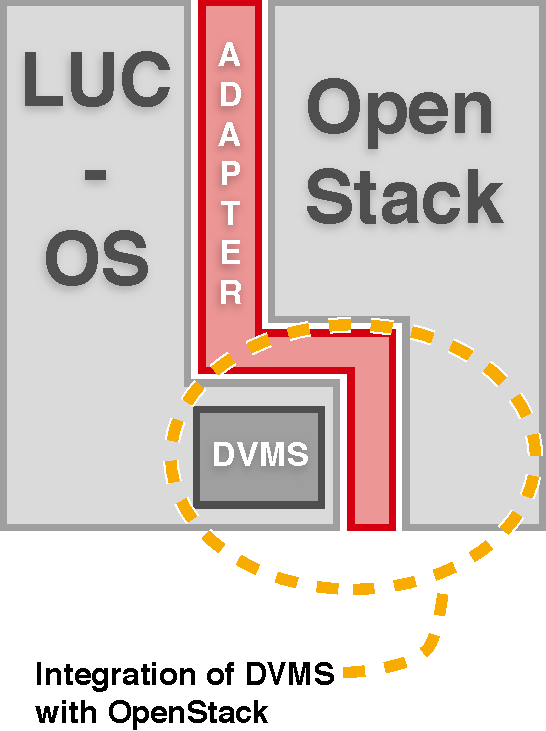
\includegraphics[width=0.50\linewidth]{Figures/dvms_openstack.pdf}
	\caption{Integration of DVMS in OpenStack.}%
	\label{fig:integration}%
	%\vspace*{-.8cm}
\end{figure}

\item Use of an "Adapter" object that will wrap DVMS and integrate well with OpenStack, as described in figure \ref{fig:integration}
	\begin{itemize}
		\item It will consume messages that are destinated to "nova-scheduler"

		\item Each message will be converted to a "Dvms" message.

		\item Each message produced by Dvms will be converted to an OpenStack message and added to the Queue.

	\end{itemize}



\end{itemize}